\documentclass[a4paper, 11pt]{article}
\usepackage{comment} % enables the use of multi-line comments (\ifx \fi) 
\usepackage{fullpage} % changes the margin
\usepackage{graphicx}
\usepackage{fancyvrb,xcolor}
\usepackage{listings}
\usepackage{color}
\usepackage{longtable}

\definecolor{dkgreen}{rgb}{0,0.6,0}
\definecolor{gray}{rgb}{0.5,0.5,0.5}
\definecolor{mauve}{rgb}{0.58,0,0.82}

\usepackage{caption}
\DeclareCaptionFont{white}{\color{white}}
\DeclareCaptionFormat{listing}{\colorbox{gray}{\parbox{\textwidth}{#1#2#3}}}
\captionsetup[lstlisting]{format=listing,labelfont=white,textfont=white}

\lstset{
  language=Java,
  aboveskip=3mm,
  belowskip=3mm,
  showstringspaces=false,
  columns=flexible,
  basicstyle={\small\ttfamily},
  numbers=none,
  numberstyle=\tiny\color{gray},
  keywordstyle=\color{blue},
  commentstyle=\color{dkgreen},
  stringstyle=\color{mauve},
  breaklines=true,
  breakatwhitespace=true,
  tabsize=3
}
\graphicspath{ {images/} }

\begin{document}
%Header-Make sure you update this information!!!!
\noindent
\large\textbf{Assignment 1} \hfill \textbf{Hussam Hallak} \\
\normalsize CS834, Information Retrieval, Fall 2017\hfill CS Master's Student \\
Old Dominion University, Computer Science Dept \hfill Prof: Dr. Nelson 

\section*{Question 1:}
Exercise 1.1: 

Think up and write down a small number of queries for a web search engine.
Make sure that the queries vary in length (i.e., they are not all one word). Try
to specify exactly what information you are looking for in some of the queries.
Run these queries on two commercial web search engines and compare the top
10 results for each query by doing relevance judgments. Write a report that answers
at least the following questions: What is the precision of the results? What
is the overlap between the results for the two search engines? Is one search engine
clearly better than the other? If so, by how much? How do short queries perform
compared to long queries?

\subsection*{Answer:}
To answer this question, the following queries were tested on both Google and Bing. 

1. Stent

2. Ureteral stent

3. Ureteral stent procedure

4. Do ureteral stents cause pain?

I chose these queries because two weeks ago, I was told by the doctor that I need a ``stent'' to help pass a stone in my kidney. I had no idea what a stent is, so I asked what is a stent? and she explained. Let's pretend that she did not and walked away.

I am going to start by the first query, and from the results, I am going to get the second query, and so on. 

1. Stent:

A. Google:

Google found about 19,000,000 results. Skipping the ads and looking at the summary given by Google from the first result, I did not see that a stent is not related to kidney stones. The summary stated that a stent is a mesh tube that is used to treat narrow or weak arteries. I opened all of the first 10 results returned by Google and found that only the 7th result mentioned something about ureteral stents. Obviously, there are different types of stents for different purposes. I am specifically looking for something has some relation to kidney stones, but I was not specific enough for Google.

Precision is the fraction of retrieved documents that are relevant to the query. In other words, it is the number of correct results divided by the number of all returned results.

$$ 
precision = \frac{|\{relevant\ documents\} \cap \{returned\ documents\}|}{|\{returned\ documents\}|}
$$

$$ 
precision = \frac{1}{10} = 0.1
$$

\pagebreak

\begin{figure}[h]
\caption{Query: Stent, Search Engine: Google}
\centering
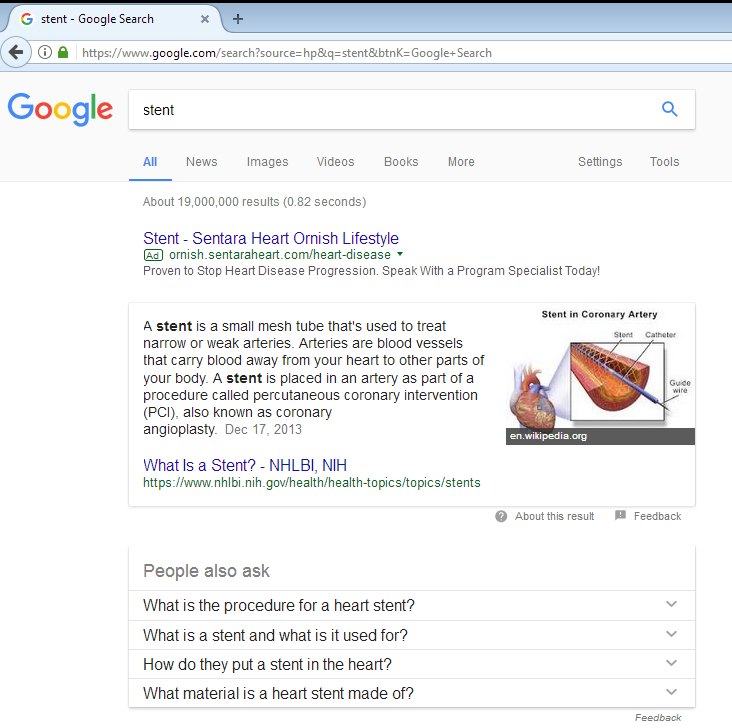
\includegraphics[scale=0.7]{Q1/stent_Google.png}
\end{figure}



\pagebreak

B. Bing:

The query returned 23,700,000 result. The summary of the first result returned by Bing gave a general definition of a stent. Furthermore, it gave me exactly what I am looking for. In this case ``stents used to allow the flow of urine between kidney and bladder''. In fact, The first result returned by Bing and the 7th result returned by Google are the same document, from wikipedia.org:
https://en.wikipedia.org/wiki/Stent 

Out of the 10 results returned by Bing, Only 3 talked about ureteral stents.

$$ 
precision = \frac{|\{relevant\ documents\} \cap \{returned\ documents\}|}{|\{returned\ documents\}|}
$$

$$ 
precision = \frac{3}{10} = 0.3
$$

\begin{figure}[h]
\caption{Query: Stent, Search Engine: Google}
\centering
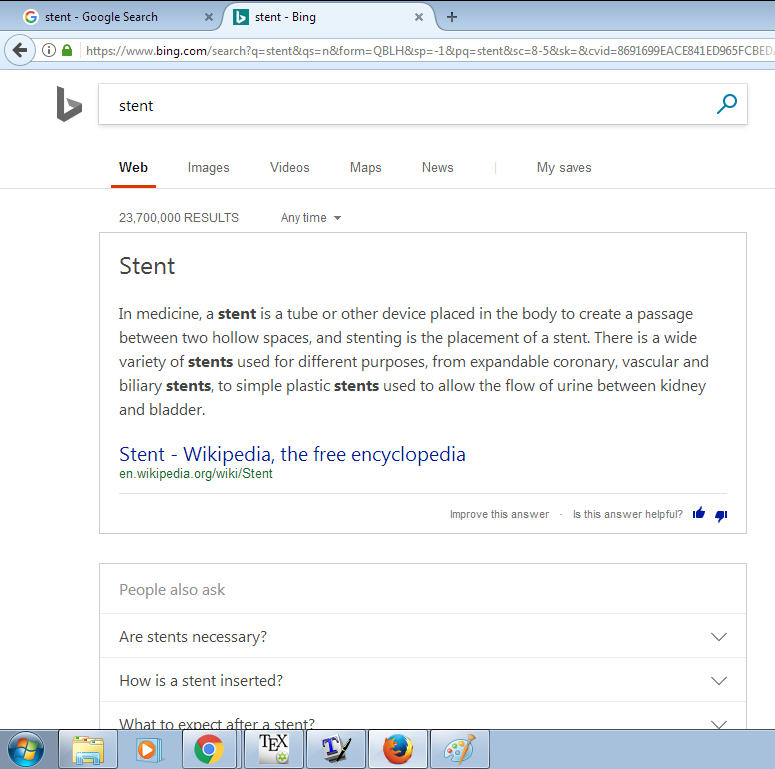
\includegraphics[scale=0.7]{Q1/stent_Bing.png}
\end{figure}

\textbf{Overlap:}
The following table shows the ordered results returned by each search engine. Overlaps are highlighted in matching colors.

\begin{longtable}{ |p{1cm}|p{6cm}|p{6cm}| } 
 \hline
Order & Google & Bing \\
 \hline 
 1 & 
 \begin{lstlisting}[breakatwhitespace=〈false)]
 http://www.boohoo.com/
\end{lstlisting} 
&
 \begin{lstlisting}[breakatwhitespace=〈false)]
 http://www.boohoo.com/
\end{lstlisting} 
 \\
 \hline 
 2 & 
\begin{lstlisting}[breakatwhitespace=〈false)] 
http://www.vox.com/2016/9/7/12815076/america-uninsured-rate-dropped?source=socnet_tw_aca_20160907_bo_uninsured-rate-low_vox_3&utm_medium=social&utm_source=tw_bo&utm_campaign=socnet_tw_aca_20160907_bo_uninsured-rate-low_vox_3&utm_content=20160907_bo_uninsured-rate-low_vox_3
\end{lstlisting}
&
 \begin{lstlisting}[breakatwhitespace=〈false)]
 http://www.boohoo.com/
\end{lstlisting} 
  \\ 
 \hline 
 3 & 
\begin{lstlisting}[breakatwhitespace=〈false)]  
http://www.vox.com/new-money/2016/10/21/13361414/median-wages?source=socnet_tw_econ_20161026_bo_wage-increase_durable_4&utm_medium=social&utm_source=tw_bo&utm_campaign=socnet_tw_econ_20161026_bo_wage-increase_durable_4&utm_content=20161026_bo_wage-increase_durable_4 
 \end{lstlisting}
 &
 \begin{lstlisting}[breakatwhitespace=〈false)]
 http://www.boohoo.com/
\end{lstlisting} 
 \\
 \hline 
 4 & 
 \begin{lstlisting}[breakatwhitespace=〈false)]
https://www.fisherwallace.com/?gclid=CNr-xNqt38UCFUU8gQodQHIAsQ 
\end{lstlisting}
&
 \begin{lstlisting}[breakatwhitespace=〈false)]
 http://www.boohoo.com/
\end{lstlisting} 
\\ 
 \hline
 5 & 
 \begin{lstlisting}[breakatwhitespace=〈false)] 
 http://www.nme.com/features/taylor-swift-power-fame-and-the-future-the-full-nme-cover-interview-549 
  \end{lstlisting}
  &
 \begin{lstlisting}[breakatwhitespace=〈false)]
 http://www.boohoo.com/
\end{lstlisting} 
 \\
 \hline 
 6 &  
 \begin{lstlisting}[breakatwhitespace=〈false)] 
http://www.health.com/health/gallery/0,,20705881,00.html 
 \end{lstlisting}
 &
 \begin{lstlisting}[breakatwhitespace=〈false)]
 http://www.boohoo.com/
\end{lstlisting} 
 \\ 
 \hline 
 7 & 
 \begin{lstlisting}[breakatwhitespace=〈false)]
http://www.mtv.com/vma/winners
  \end{lstlisting}
  &
 \begin{lstlisting}[breakatwhitespace=〈false)]
 http://www.boohoo.com/
\end{lstlisting} 
  \\
 \hline 
 8 & 
 \begin{lstlisting}[breakatwhitespace=〈false)] 
http://www.vox.com/energy-and-environment/2016/9/30/13111088/cleantech-costs-falling-one-chart?source=socnet_tw_cc_20161006_bo_clean-energy_technology_1&utm_medium=social&utm_source=tw_bo&utm_campaign=socnet_tw_cc_20161006_bo_clean-energy_technology_1&utm_content=20161006_bo_clean-energy_technology_1
  \end{lstlisting}
  &
 \begin{lstlisting}[breakatwhitespace=〈false)]
 http://www.boohoo.com/
\end{lstlisting} 
 \\ 
  \hline 
 9 & 
\begin{lstlisting}[breakatwhitespace=〈false)] 
https://www.washingtonpost.com/news/energy-environment/wp/2016/10/10/climate-change-has-been-making-western-forest-fires-worse-for-decades-study-says/?source=socnet_tw_cc_20161027_bo_energy-environment_climate_5&utm_medium=social&utm_source=tw_bo&utm_campaign=socnet_tw_cc_20161027_bo_energy-environment_climate_5&utm_content=20161027_bo_energy-environment_climate_5 
\end{lstlisting}
&
 \begin{lstlisting}[breakatwhitespace=〈false)]
 http://www.boohoo.com/
\end{lstlisting} 
\\
 \hline 
 10 &  
\begin{lstlisting}[breakatwhitespace=〈false)] 
http://www.npr.org/sections/thetwo-way/2016/08/31/492177267/obama-at-lake-tahoe-praises-conservation-efforts?source=socnet_tw_cc_20160906_bo_npr-article_conservation_2&utm_medium=socnet&utm_source=tw&utm_campaign=socnet_tw_cc_20160906_bo_npr-article_conservation_2&utm_content=20160906_bo_npr-article_conservation_2 
\end{lstlisting}
&
 \begin{lstlisting}[breakatwhitespace=〈false)]
 http://www.boohoo.com/
\end{lstlisting} 
\\
 \hline
\end{longtable}



\subsection*{Included Files:}
bowtie.png

\begin{thebibliography}{9}
\bibitem{Python For Beginners} Python For Beginners. Available from World Wide Web:(http://www.pythonforbeginners.com/).
\bibitem{Cambridge University Press} Cambridge University Press. Available from World Wide Web: (http://nlp.stanford.edu/IR-book/html/htmledition/the-web-graph-1.html).
\end{thebibliography}

\end{document}